To create environments for the web navigation tasks, we generate synthetic websites that agents must learn to navigate. These websites serve as training and evaluation environments, where agents need to fill forms and interact with various web elements. Here we describe our procedural website generation process.

To generate the set of websites $W$, we first assume a target number of websites, denoted as $N_{\text{websites}}$.
Following the approach in \citet{gur2021environment} (shown in Table 4 of the paper), we consider 42 possible primitives that can be added to a web page and introduce two additional primitives: a "new page" primitive and a "stop" primitive, resulting in a total of 44 primitives.

The website generation process begins with an empty web page.
We repeatedly sample uniformly from the 44 primitives and add them to the current page.
If the "new page" primitive is selected during the sampling process, we start adding primitives to a new linked page.
If the "stop" primitive is selected, we conclude the generation of the current website and proceed to generate the next website, if necessary.
This process continues until we have generated the desired number of websites, $N_{\text{websites}}$.
Each website in the resulting set $W$ consists of one or more web pages, with each page containing a sampled set of primitives.

We define the difficulty of a web page as the probability of a random agent interacting with the correct primitive(s).
The difficulty of page $p_i$ is given by $-\log \left (\frac{n_{\text{active}}}{n_\text{active}+n_\text{passive}} \right )$, where $n_{\text{active}}$ and $n_{\text{passive}}$ denote the number of active and passive primitives on the page, respectively.
The difficulty of an entire sequence of web pages is determined by summing the difficulty of all individual pages it contains.
Based on these difficulty calculations, we partition the websites into three difficulty levels.
The three levels of difficulty correspond to the probability thresholds of 50\%, 25\%, and 10\% for levels 1, 2, and 3, respectively.
Users can select a specific difficulty level of web navigation by executing Python commands such as \verb|env = gym.make("WebNavigation-Difficulty-01-v0", num_websites=1)|, where the \verb|num_websites| argument defines the pool of websites available for the environment. During training or evaluation, each episode begins by randomly selecting one website from this pool at the specified difficulty level. For example, if \verb|num_websites=10|, the environment will generate 10 websites at the specified difficulty level, and each episode will randomly assign one of these websites for the agent to navigate.
At each timestep, the agent can interact with an HTML element on the page, such as modifying the text field or clicking on the element, with the objective of entering correct information into forms and clicking "next" or "submit" to advance between web pages.

% To generate the initial set $P$ of web pages, we first determined the number of pages $N_{\text{pages}}$, such that $|P| = N_{\text{pages}}$, and set the maximum number of primitives per page as $N_{\text{prim}}$. Following the approach in~\cite{gur2021environment} (Table 4), we selected 42 possible primitives to be added to a blank web page. Next, we uniformly sampled a random number of primitives between 0 and $N_{\text{prim}}$, and added these selected primitives to the page. This process resulted in a collection of single web pages, each with a distinct configuration of primitives.
% After generating the pages, we proceeded to create a set of websites, denoted by $W$. Initially, we set $W$ equal to $P$. We then generated additional web pages by randomly selecting two websites, $w_i$ and $w_j$, from $W$, and linking the final page of $w_i$ to the first page of $w_j$. Since gMiniWob currently only supports single connections between pages, passive primitives on a page terminate the interaction, while active primitives allow the agent to continue filling out the web form.
% For pages without sampled active primitives, an active primitive (submit button) is added to ensure that the agent can proceed.

% After generating a fixed number of websites, we partitioned these websites into three difficulty levels. For instance, users can select a specific difficulty level of web navigation by executing Python commands such as \texttt{env = gym.make('WebNavigation-v0', difficulty=1, num\_websites=1)}, where the \texttt{num\_websites} argument defines the number of websites that are generated for this environment.
% Ranking the websites by difficulty was done by analysing the performance of random agents. The three levels of difficulty are defined by a random agent successfully completing a website with a probability higher than \% 50, \% 25 and \%10 percent for levels 1, 2 and 3 respectively.
% To address this, we defined the difficulty of a web page as the probability of interacting with the correct primitive(s).
% The difficulty of page $p_i$ is then given by $- \log \left (\frac{n_{\text{active}}}{n_\text{active}+n_\text{passive}} \right )$, where $n_{\text{active}}$ and $n_{\text{passive}}$ denote the number of active and passive primitives on the page, respectively.
% The difficulty of an entire sequence of web pages is determined by summing the difficulty of all individual pages it contains.

% At each timestep, the agent can interact with an HTML element on the page, such as modifying the text field or clicking on the element, with the objective of entering correct information into forms and clicking "next" or "submit" to advance between webpages.

% \begin{figure}[H]
%     \centering
%     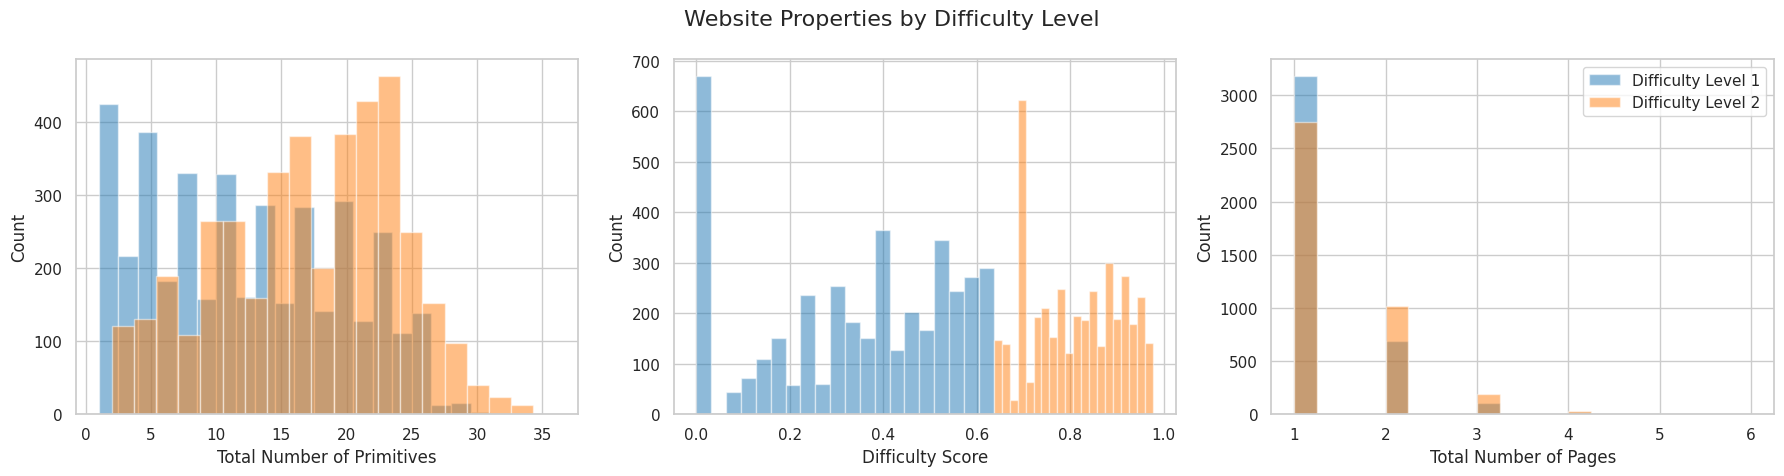
\includegraphics[width=\linewidth]{img/web_nav/website_properties_difficulty_levels_1_2.png}
%     % \caption{Caption}
%     \label{fig:enter-label1}
% \end{figure}
% \vspace{-1.10cm}
% \begin{figure}[H]
%     \centering
%     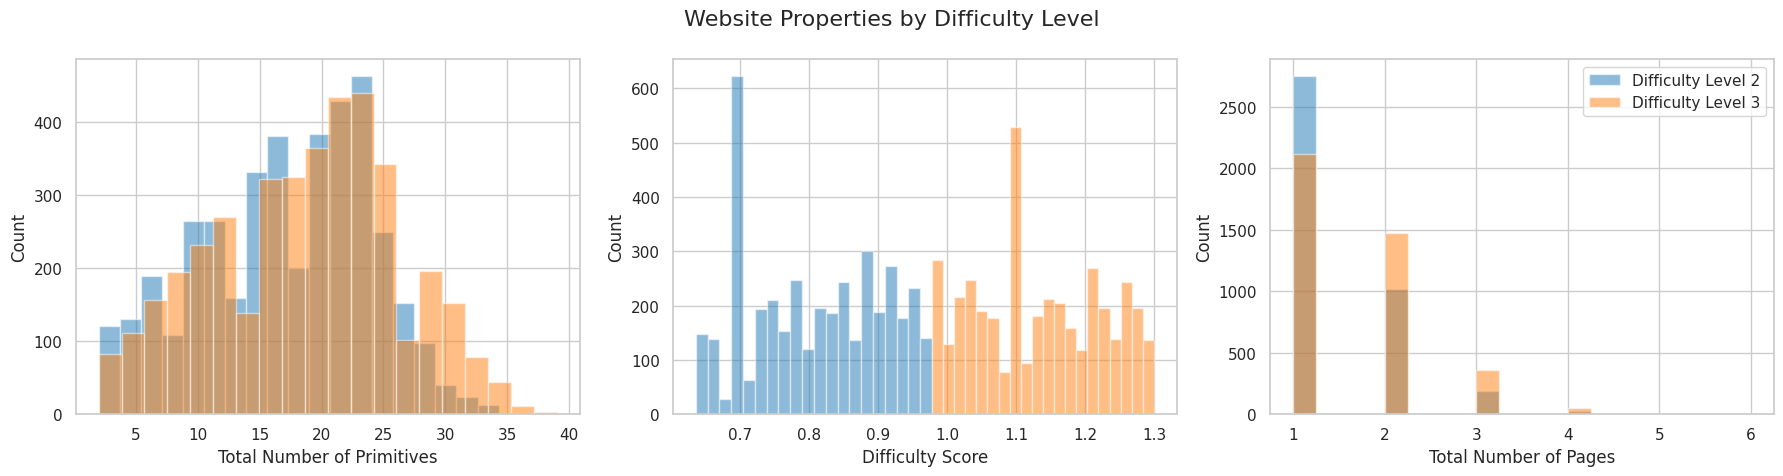
\includegraphics[width=\linewidth]{img/web_nav/website_properties_difficulty_levels_2_3.png}
%     % \caption{Caption}
%     \label{fig:enter-label2}
% \end{figure}
% \vspace{-1.10cm}

% \begin{figure}[H]
%     \centering
%     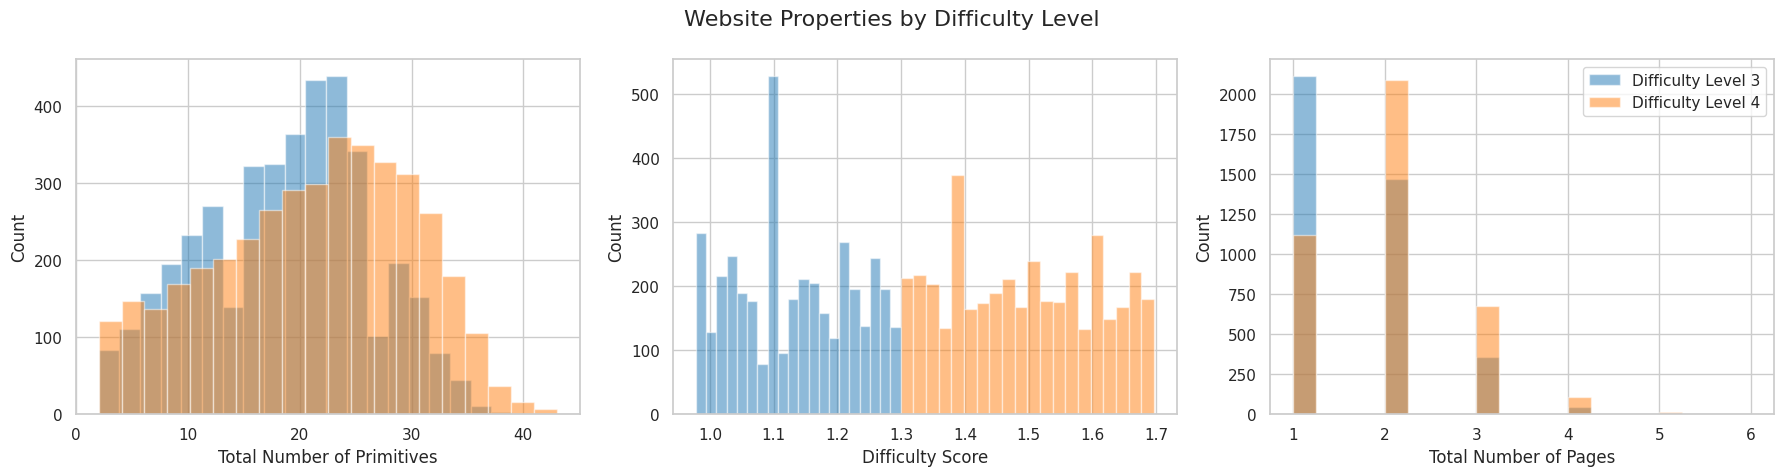
\includegraphics[width=\linewidth]{img/web_nav/website_properties_difficulty_levels_3_4.png}
%     % \caption{Caption}
%     \label{fig:enter-label3}
% \end{figure}
% \vspace{-1.10cm}

% \begin{figure}[H]
%     \centering
%     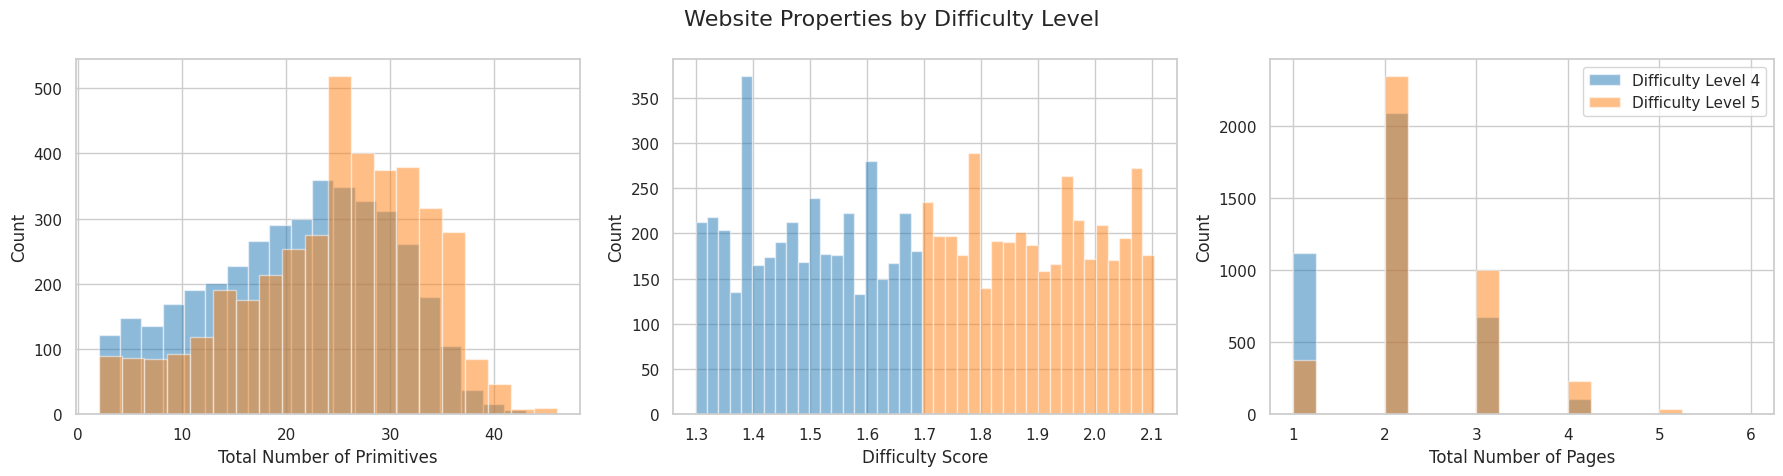
\includegraphics[width=\linewidth]{img/web_nav/website_properties_difficulty_levels_4_5.png}
%     % \caption{Caption}
%     \label{fig:enter-label4}
% \end{figure}
% \vspace{-1.10cm}

% \begin{figure}[H]
%     \centering
%     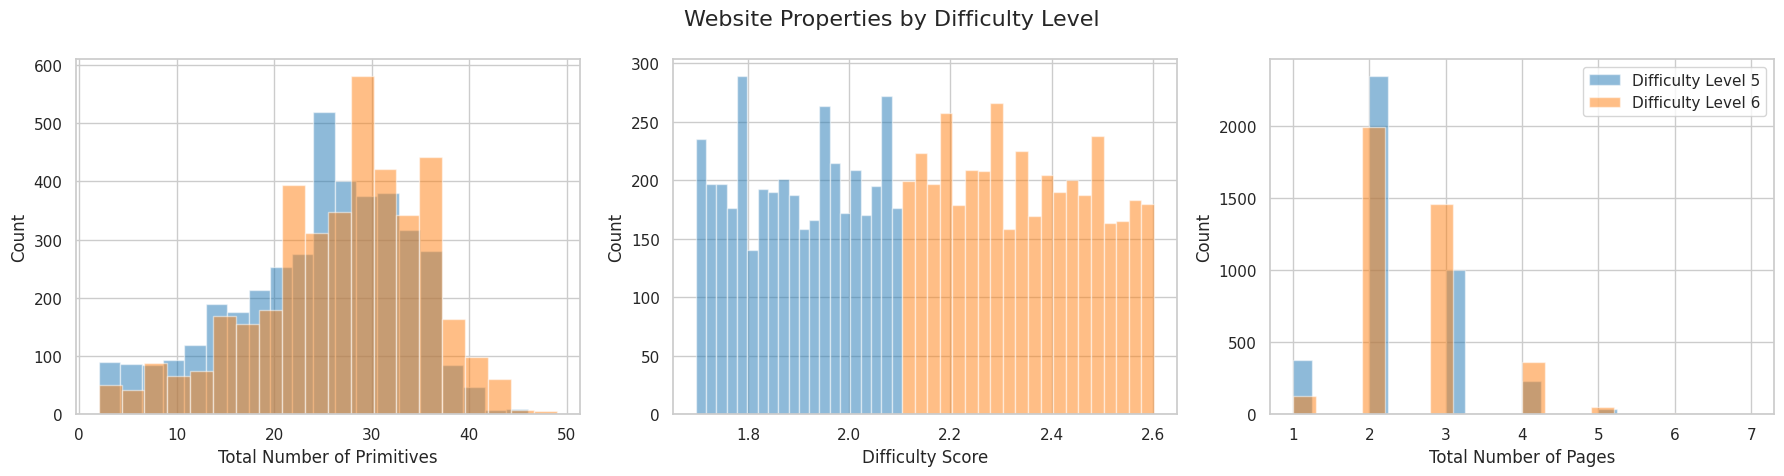
\includegraphics[width=\linewidth]{img/web_nav/website_properties_difficulty_levels_5_6.png}
%     % \caption{Caption}
%     \label{fig:enter-label5}
% \end{figure}
% \vspace{-1.10cm}

% \begin{figure}[H]
%     \centering
%     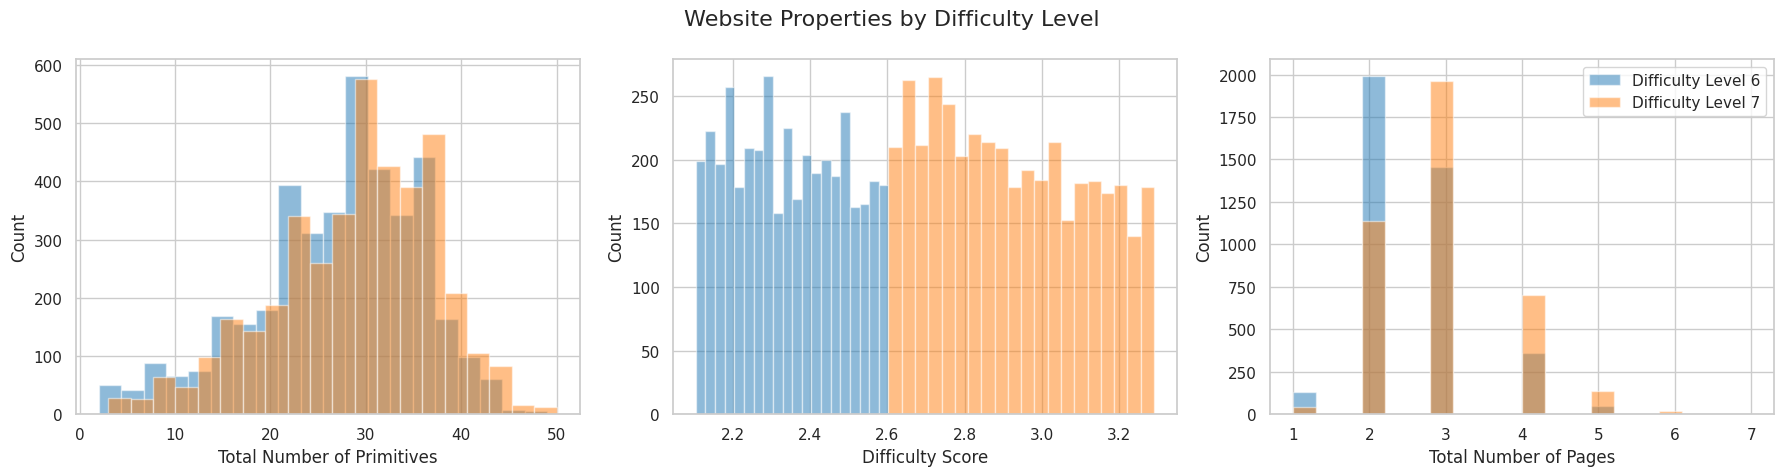
\includegraphics[width=\linewidth]{img/web_nav/website_properties_difficulty_levels_6_7.png}
%     % \caption{Caption}
%     \label{fig:enter-label6}
% \end{figure}
% \vspace{-1.10cm}

% \begin{figure}[H]
%     \centering
%     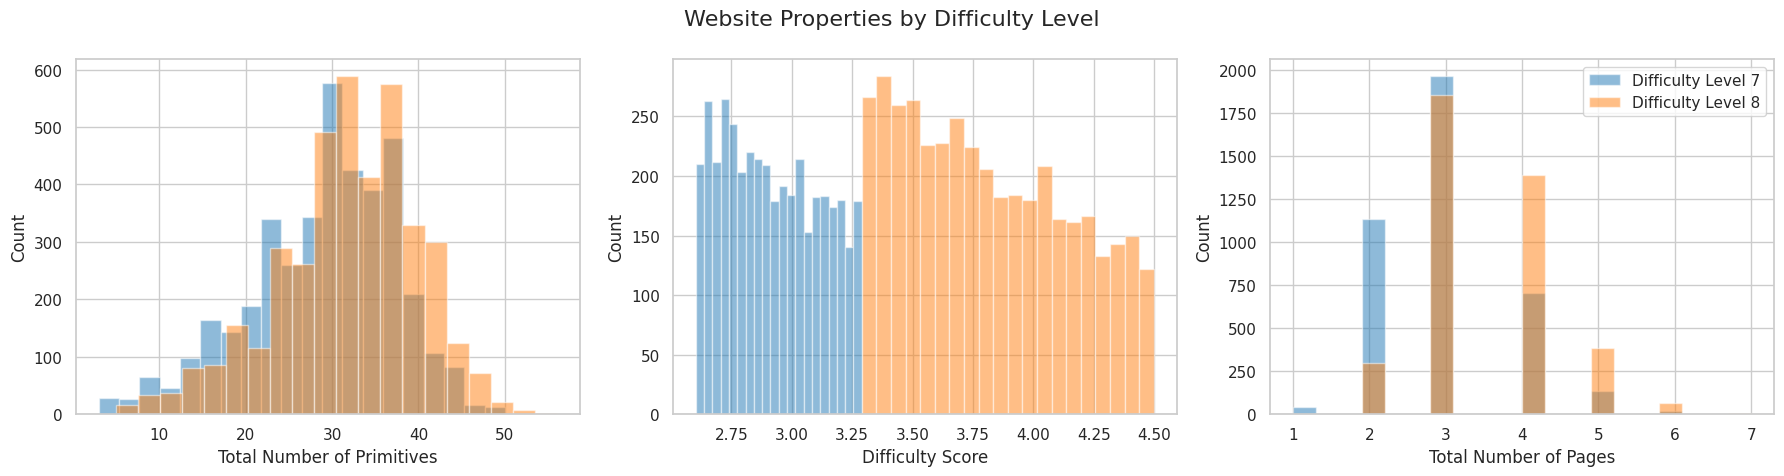
\includegraphics[width=\linewidth]{img/web_nav/website_properties_difficulty_levels_7_8.png}
%     % \caption{Caption}
%     \label{fig:enter-label7}
% \end{figure}
% \vspace{-1.10cm}

% \begin{figure}[H]
%     \centering
%     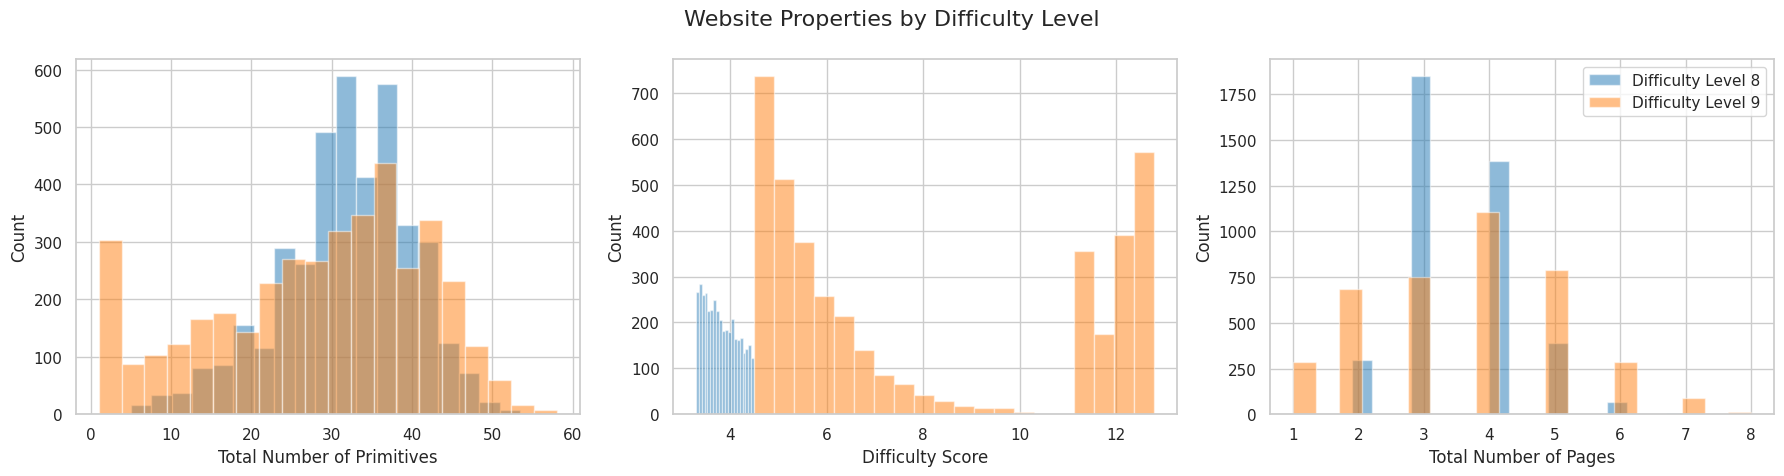
\includegraphics[width=\linewidth]{img/web_nav/website_properties_difficulty_levels_8_9.png}
%     % \caption{Caption}
%     \label{fig:enter-label8}
% \end{figure}
